\section{Hasil \textit{Rebalancing} Strategi}
\label{sec:4_11_window_analysis}

Proses \textit{rebalance} atau penyeimbangan ulang portofolio merupakan prosedur investasi dengan menjalankan algoritma strategi setiap periode waktu tertentu untuk menyesuaikan alokasi portofolio. Karena pada dasarnya, alokasi aset akan berubah sesuai dengan perubahan harga aset yang dipilih oleh investor melalui strategi yang digunakan. Dalam metode yang digunakan pada tugas akhir ini, periode waktu \textit{rebalance} dilakukan setiap bulan dengan tetap menggunakan pelatihan data 6 bulan atau 1 semester. \textit{Rebalance} dilakukan dengan simulasi yang sama yaitu dengan pembaruan Hamiltonian dari data historis dalam runtun waktu 6 bulan terbaru di setiap (\textit{window}) atau jendela simulasi. Algoritma diawali dengan mengekstraksi matriks korelasi dan imbal hasil ekspektasian terkini, kemudian dikonversi menjadi parameter bias lokal ($h_i$) dan interaksi kopling ($J_{ij}$) pada operator Hamiltonian sistem. Perubahan nilai parameter tersebut akan merubah lanskap energi, di mana (\textit{ground state}) dapat bergeser dari satu konfigurasi spin ke konfigurasi lainnya sehingga akan terkadang akan menyebabkan pemilihan aset yang berbeda dari sebelumnya. Namun jika pemilihan aset tetap sama, alokasi asetnya akan dikembalikan menjadi 50\% modal untuk setiap aset pada sistem N=4.

Hasil \textit{rebalancing} dapat teramati lewat grafik pertumbuhan aset pada gambar \ref{fig:compare_vqe_classic} yang mana terlihat ada tekanan \textit{drawdown} atau penurunan nilai investasi pada awal pertumbuhan aset. Tekanan tersebut dapat teramati pada transisi (\textit{window}) Februari--Maret 2021 sehingga mengakibatkan dinamika algoritma pada Gambar \ref{fig:window_n4_2021_02_02} dan Gambar \ref{fig:window_n4_2021_03_04} di Lampiran \ref{appendix:window_analysis_n4} dengan rangkaian untuk iterasi terakhir pada Gambar \ref{fig:circuit_n4_2021_02_02} dan Gambar \ref{fig:circuit_n4_2021_03_04} di Lampiran \ref{appendix:circuit_performance_n4}. Pada periode tersebut, terjadi lonjakan risiko pada sektor telekomunikasi (TLKM) yang direpresentasikan oleh penurunan parameter bias objek pada Hamiltonian. Untuk merespons hal tersebut, sirkuit kuantum melakukan rotasi parameter sudut $\theta$ secara signifikan agar amplitudo probabilitas dapat dipindahkan dari status $|0110\rangle$ menuju status $|0011\rangle$. Mekanisme tersebut menunjukkan bahwa strategi hibrida memiliki agilitas cukup tinggi dalam mengeksplorasi parameter $\theta$ agar memperoleh energi paling efisien tanpa harus terkendala hambatan komputasi klasik. Selain itu, terdapat dampak  signifikan pada stabilitas \textit{warm-start} yang mana terlihat kedalaman sirkuit yang dipilih dominan lebih rendah untuk keseluruhan \textit{window}. Berdasarkan laporan tersebut, 

\begin{figure}[!htbp]
    \centering
    \begin{subfigure}[b]{0.45\textwidth}
        \centering
        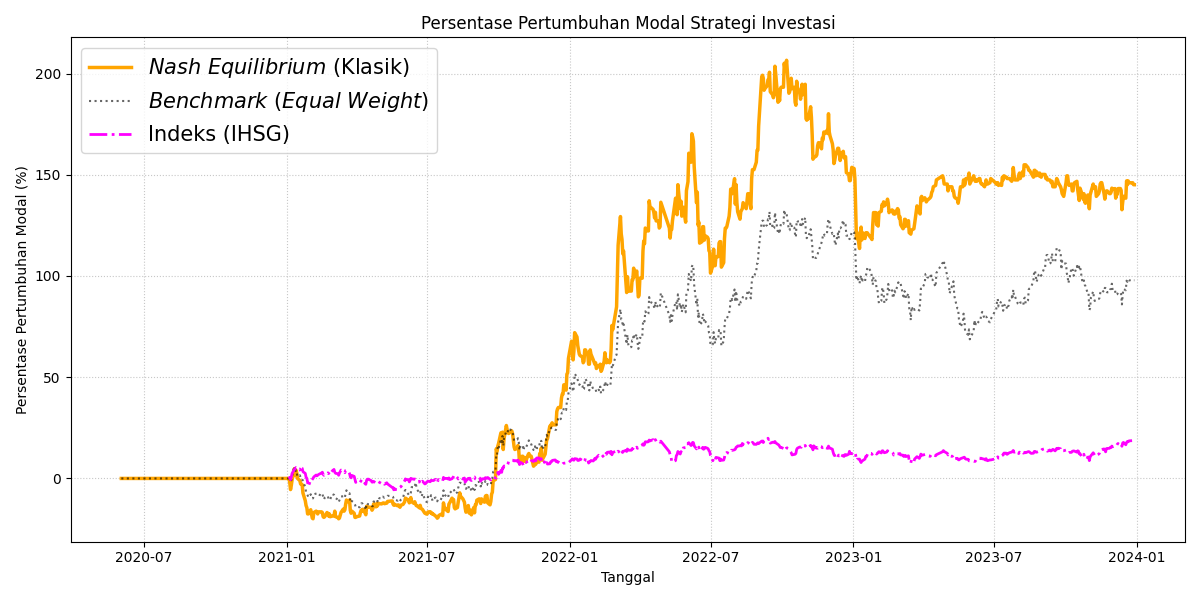
\includegraphics[width=\textwidth]{GTQuantumInvest/Hasil_N2_GT/hasil_backtest_nash_N2.png}
        \caption{Strategi \textit{Nash} (Klasik)}
    \end{subfigure}
    \hfill
    \begin{subfigure}[b]{0.45\textwidth}
        \centering
        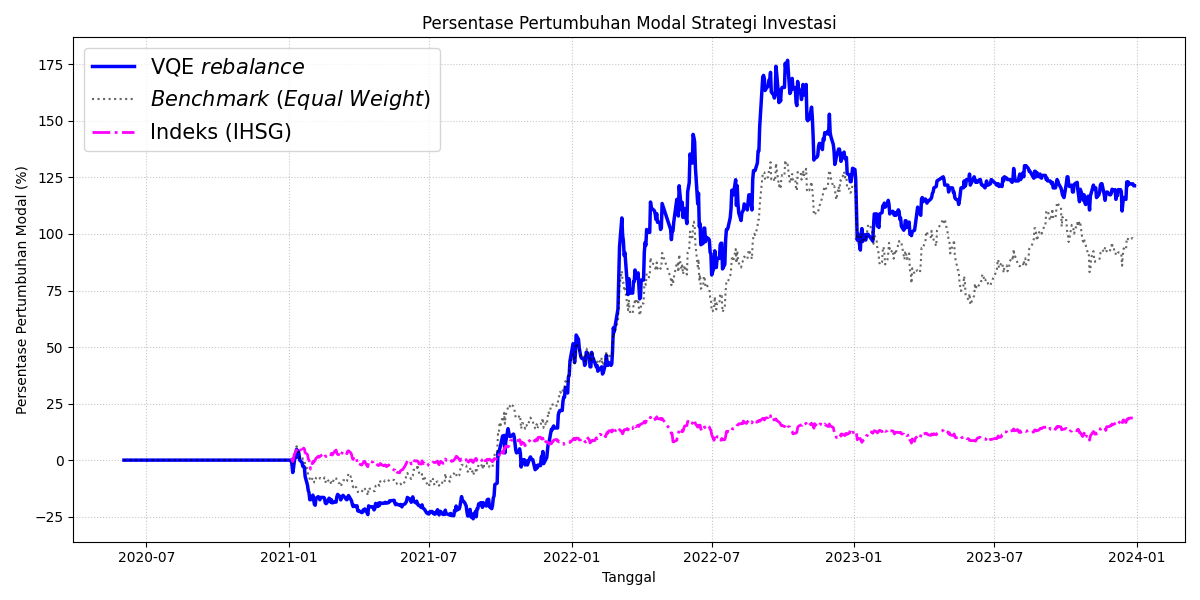
\includegraphics[width=\textwidth]{GTQuantumInvest/Hasil_N2_NoGT/hasil_backtest_vqe_N2.png}
        \caption{VQE (Tanpa \textit{Game Theory})}
    \end{subfigure}
    \caption{Perbandingan Performa Portofolio Klasik vs Kuantum Murni pada Sistem N=2.}
    \label{fig:comp_n2_base}
\end{figure}

\begin{figure}[!htbp]
    \centering
    \begin{subfigure}[b]{0.45\textwidth}
        \centering
        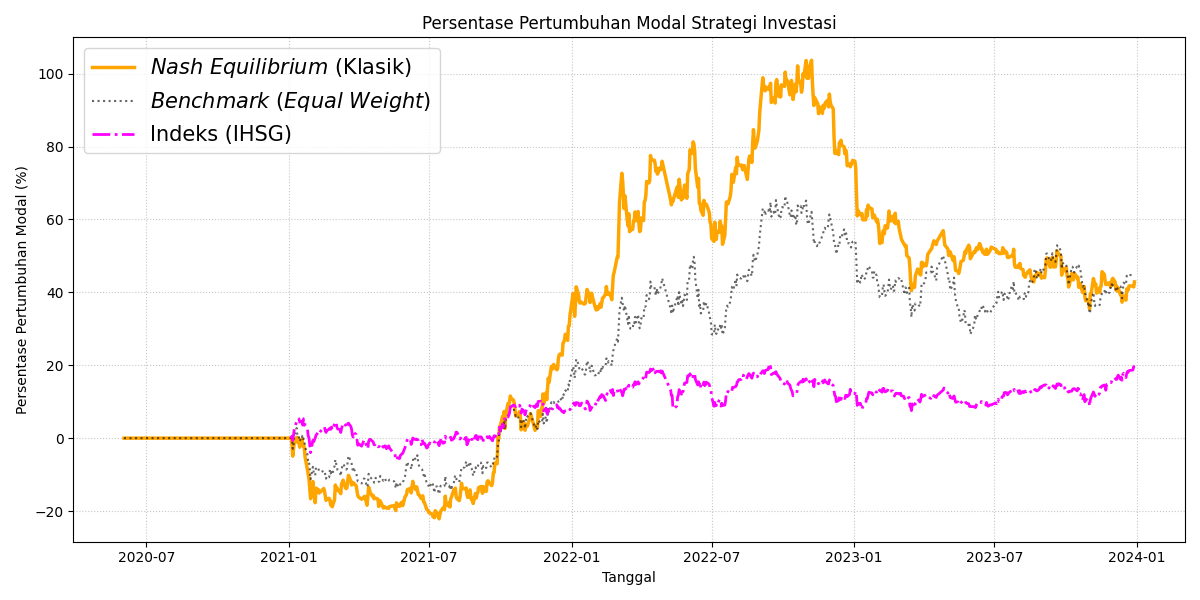
\includegraphics[width=\textwidth]{GTQuantumInvest/Hasil_N4_GT/hasil_backtest_nash_N4.png}
        \caption{Strategi \textit{Nash} (Klasik)}
    \end{subfigure}
    \hfill
    \begin{subfigure}[b]{0.45\textwidth}
        \centering
        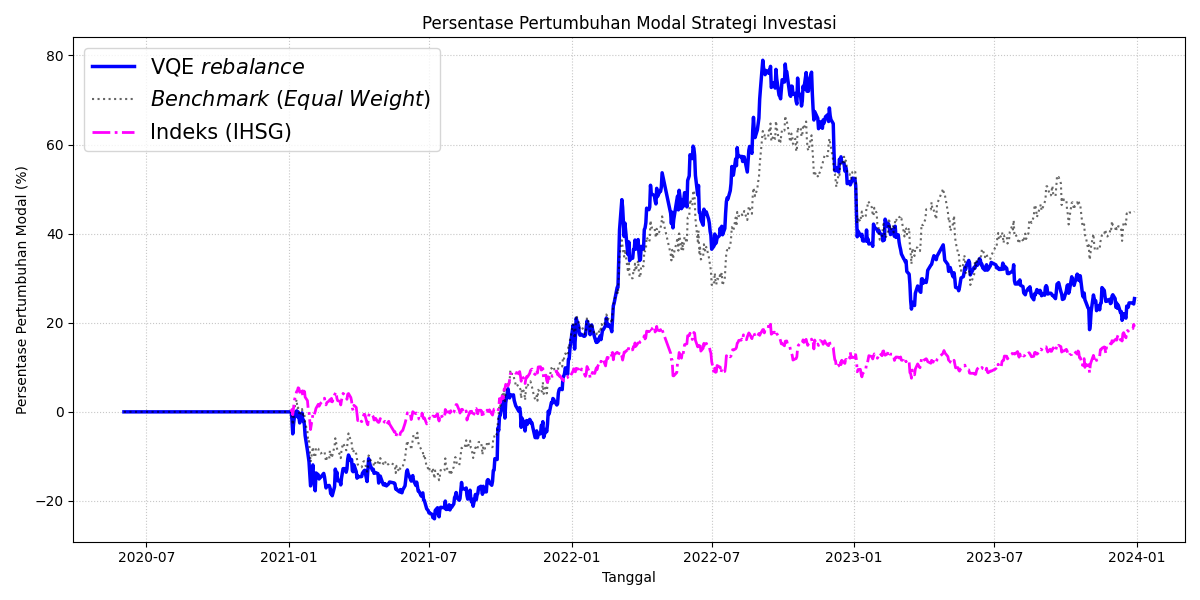
\includegraphics[width=\textwidth]{GTQuantumInvest/Hasil_N4_NoGT/hasil_backtest_vqe_N4.png}
        \caption{VQE (Tanpa \textit{Game Theory})}
    \end{subfigure}
    \caption{Perbandingan Performa Portofolio Klasik vs Kuantum Murni pada Sistem N=4.}
    \label{fig:comp_n4_base}
\end{figure}

Secara kumulatif, efektivitas mekanisme \textit{rebalancing} hibrida ini menghasilkan kurva pertumbuhan modal yang stabil dan \textit{outperform} dari strategi pembandignya. Perbandingan pada Gambar \ref{fig:comp_n2_base} dan \ref{fig:comp_n4_base} menunjukkan bahwa tanpa integrasi kecerdasan strategis, performa VQE murni cenderung tertahan atau bahkan mengalami degradasi saat dimensi sistem membesar. Namun, dengan integrasi \textit{Game Theory} (GT) sebagai inisialisasi keadaan, sirkuit mampu mempertahankan integritas solusinya. Hal ini dapat terbukti juga pada visualisasi Gambar \ref{fig:rebalancing_impact} yang menunjukkan pertumbuhan modal konsisten pada kedua konfigurasi sistem. Oleh karena itu, algoritma ini mampu melindungi nilai portofolio dari potensi (\textit{drawdown}) yang sangat dalam dengan mendeteksi secara dini bagaimana pergeseran ekuilibrium pasar yang terjadi ke dalam dinamika fisis yang dimikiliki oleh sirkuit kuantum.

\begin{figure}[!htbp]
    \centering
    \begin{subfigure}[b]{0.45\textwidth}
        \centering
        
\includegraphics[width=\textwidth]{GTQuantumInvest/Hasil_N2_GT/hasil_backtest_vqe_N2.png}
        \caption{Performa GT-VQE ($N=2$)}
    \end{subfigure}
    \hfill
    \begin{subfigure}[b]{0.45\textwidth}
        \centering
        
\includegraphics[width=\textwidth]{GTQuantumInvest/Hasil_N4_GT/hasil_backtest_vqe_N4.png}
        \caption{Performa GT-VQE ($N=4$)}
    \end{subfigure}
    \caption{Perbandingan Visual Pertumbuhan Modal pada Sistem N=2 dan N=4 sebagai Hasil dari Algoritma \textit{Rebalancing} Strategis.}
    \label{fig:rebalancing_impact}
\end{figure}
